\documentclass[../../main.tex]{subfiles}
\graphicspath{{../../image/}{../../figure/}}
\begin{document}

\section{解的唯一性}\label{section:ch14-解的唯一性}

Cauchy 问题\eqref{align:ch13-ivp}的唯一性将在此通过证明任一合理函数类中的解可等同于从初值发出的标准 Riemann 半群轨道而建立。如\cref{section:ch14-标准riemann半群}所示，对前沿追踪构造的解确实如此。



为公平比较，一开始就把研究限制为 $U(\cdot,t)$ 位于标准 Riemann 半群定义域 $\mathscr{D}$（通过\eqref{align:ch14-domain}定义）中的解 $U$。如前所述，这特别蕴含 $U(\cdot,t)$ 在 $(-\infty,\infty)$ 上有有界变差：
\begin{align}
TV_{(-\infty,\infty)}U(\cdot,t)\leqslant cr.
\label{align:ch14-un-TV}
\end{align}
继而由\cref{theorem:ch04-BV时间Lipschitz}，$t\mapsto U(\cdot,t)$ 是 $L^1$-Lipschitz 的，
\begin{align}
\int_{-\infty}^\infty|U(x,t)-U(x,\tau)|\,\mathrm{d}x\leqslant c'r|t-\tau|,\qquad 0\leqslant\tau<t<\infty,
\label{align:ch14-un-lip}
\end{align}
且 $U$ 在 $(-\infty,\infty)\times[0,\infty)$ 上属于 $BV_{\mathrm{loc}}$。因而如\cref{section:ch10-bv解}所指出，存在零测集 $\mathscr{N}\subset[0,\infty)$，使任一满足 $t\notin\mathscr{N}$ 且 $U(x-,t)=U(x+,t)$ 的 $(x,t)$ 是 $U$ 的近似连续点，而任一满足 $t\notin\mathscr{N}$ 且 $U(x-,t)\neq U(x+,t)$ 的 $(x,t)$ 是 $U$ 的近似跳跃间断点，具有单侧近似极限 $U_\pm=U(x\pm,t)$ 及由 Rankine--Hugoniot 跳跃条件\eqref{align:ch08-rh}确定的相应激波速度。



目前尚不清楚唯一性是否在上述解类中成立。因而应对解赋予额外结构。这里我们试验：

\begin{definition}[ tame 振荡条件]\label{definition:ch14-tame振荡条件}
存在正常数 $\lambda$ 与 $\beta$，使对所有 $x\in(-\infty,\infty)$、$t\in[0,\infty)$ 与任一 $h>0$，
\begin{align}
|U(x\pm,t+h)-U(x\pm,t)|\leqslant\beta\,TV_{(x-\lambda h,x+\lambda h)}U(\cdot,t).
\label{align:ch14-tame}
\end{align}
\end{definition}

显然，由随机选择法或前沿追踪算法构造的解满足此条件，\cref{chapter:ch12-两方程真非线性组}中所考虑的两个守恒律系统的解亦然。



tame 振荡条件诱导唯一性：

\begin{theorem}\label{theorem:ch14-唯一性}
设 $U$ 是 Cauchy 问题\eqref{align:ch13-ivp}的任一 $BV$ 解，$U(\cdot,t)\in\mathscr{D}$ 对所有 $t\in[0,\infty)$ 成立，在任一近似跳跃间断点满足 Lax $E$-条件，并满足 tame 振荡条件\eqref{align:ch14-tame}，则 $U$ 与从初值发出的标准 Riemann 半群 $S_t$ 的轨道重合：
\begin{align}
U(\cdot,t)=S_tU_0(\cdot),\qquad t\in[0,\infty).
\label{align:ch14-un-trajectory}
\end{align}
特别地，$U$ 由其初值唯一确定。
\end{theorem}



\begin{proof}
证明相当冗长。第一步是证明在每个 $\tau\notin\mathscr{N}$，$U(\cdot,t)$ 与从 $U(\cdot,\tau)$ 发出的 $S_t$ 轨道相切：
\begin{align}
\limsup_{h\downarrow0}\frac1h\|U(\cdot,\tau+h)-S_hU(\cdot,\tau)\|_{L^1(-\infty,\infty)}=0.
\label{align:ch14-tangent}
\end{align}
接着验证\eqref{align:ch14-tangent}转而蕴含\eqref{align:ch14-un-trajectory}。

固定 $\tau\notin\mathscr{N}$，我们通过如下过程建立\eqref{align:ch14-tangent}。对任一固定有界区间 $[a,b]$ 与任意小 $\varepsilon>0$，在矩形 $[a,b]\times[\tau,\tau+\delta]$ 上构造某函数 $U^*$，使
\begin{align}
\limsup_{h\downarrow0}\frac1h\|U(\cdot,\tau+h)-U^*(\cdot,h)\|_{L^1(a,b)}\leqslant c_{14}r\varepsilon,
\label{align:ch14-Ustar1}
\end{align}
\begin{align}
\limsup_{h\downarrow0}\frac1h\|S_hU(\cdot,\tau)-U^*(\cdot,h)\|_{L^1(a,b)}\leqslant c_{14}r\varepsilon.
\label{align:ch14-Ustar2}
\end{align}
自然地，此种 $U^*$ 将提供初值 $U_0(\cdot)=U(\cdot,\tau)$ 的\eqref{align:ch13-ivp}解的局部逼近，并相应地通过拼接两类局部近似解构造：一类适合强跳跃间断点，另一类适合小局部振荡区域。



我们先固定 $\lambda$，它大于所有特征速度的绝对值，且充分大使 tame 振荡条件\eqref{align:ch14-tame}可应用。

对 $U$ 的任一跳跃间断点 $(y,\tau)$，具有极限 $U_\pm=U(y\pm,\tau)$ 与激波速度 $s$，我们关联扇区 $\mathscr{K}=\{(x,\sigma):\sigma>0,\ |x-y|\leqslant\lambda\sigma\}$，在其上考虑由
\begin{align}
U^\sharp(x,\sigma)=
\begin{cases}
U_-, & x<y+s\sigma,\\
U_+, & x>y+s\sigma
\end{cases}
\label{align:ch14-sector}
\end{align}
定义的解 $U^\sharp=U^\sharp_{(y,\tau)}$。我们证明
\begin{align}
\lim_{h\downarrow0}\frac1h\int_{y-\lambda h}^{y+\lambda h}|U(x,\tau+h)-U^\sharp(x,h)|\,\mathrm{d}x=0.
\label{align:ch14-sector-limit}
\end{align}
确实，对 $0\leqslant\sigma\leqslant h$，置
\begin{align}
\phi_h(\sigma)=\frac1h\int_{y-\lambda h}^{y+\lambda h}|U(x,\tau+\sigma)-U^\sharp(x,\sigma)|\,\mathrm{d}x.
\label{align:ch14-phi}
\end{align}
设 $\phi_h(h)>0$。由于 $\sigma\mapsto U(\cdot,\tau+\sigma)-U^\sharp(\cdot,\sigma)$ 是 $L^1$-Lipschitz 的，常数为 $\gamma$，我们推得对 $h\ll1$，$\phi_h(h)<2\gamma$，且对任一满足 $h-\sigma\leqslant\frac{h}{2\gamma}\phi_h(h)$ 的 $\sigma$，$\phi_h(\sigma)\geqslant\frac12\phi_h(h)$。于是
\begin{align}
\frac{1}{h^2}\int_0^h\int_{y-\lambda h}^{y+\lambda h}|U(x,\tau+\sigma)-U^\sharp(x,\sigma)|\,\mathrm{d}x\,\mathrm{d}\sigma=\frac1h\int_0^h\phi_h(\sigma)\,\mathrm{d}\sigma\geqslant\frac{1}{4\gamma}\phi_h^2(h).
\label{align:ch14-sector-integral}
\end{align}
当 $h\downarrow0$ 时，由\cref{theorem:ch01-BV链式法则}，\eqref{align:ch14-sector-integral}左端趋于零，这验证了\eqref{align:ch14-sector-limit}。



接着固定任一区间 $(\zeta,\xi)$，中点设为 $z$。在三角区域 $\mathscr{T}=\{(x,\sigma):\sigma>0,\ \zeta+\lambda\sigma<x<\xi-\lambda\sigma\}$ 上，构造线性 Cauchy 问题的解 $U^\flat=U^\flat_{(z,\tau)}$：
\begin{align}
\partial_t U^\flat+A^\flat\partial_x U^\flat=0,
\label{align:ch14-linear-pde}
\end{align}
\begin{align}
U^\flat(x,0)=U(x,\tau),
\label{align:ch14-linear-ic}
\end{align}
其中 $A^\flat$ 是常矩阵 $DF(U(z,\tau))$。目的是建立估计
\begin{align}
\int_{\zeta+\lambda h}^{\xi-\lambda h}|U(x,\tau+h)-U^\flat(x,h)|\,\mathrm{d}x\leqslant c_{15}[TV_{(\zeta,\xi)}U(\cdot,\tau)]\int_0^h TV_{(\zeta+\lambda\sigma,\xi-\lambda\sigma)}U(\cdot,\tau+\sigma)\,\mathrm{d}\sigma.
\label{align:ch14-linear-est}
\end{align}

沿特征方向积分\eqref{align:ch14-linear-pde}并利用\eqref{align:ch14-linear-ic}给出
\begin{align}
L_i^\flat U^\flat(x,h)=L_i^\flat U(x-\lambda_i^\flat h,\tau),\qquad i=1,\cdots,n,
\label{align:ch14-char}
\end{align}
其中 $L_i^\flat=L_i(U(z,\tau))$ 是 $A^\flat$ 的与特征值 $\lambda_i^\flat=\lambda_i(U(z,\tau))$ 相应的左特征向量。对固定 $i$，可不失一般性假设 $\lambda_i^\flat=0$，因为可作变量替换 $x\mapsto x-\lambda_i^\flat t$、$F(U)\mapsto F(U)-\lambda_i^\flat U$。此情形下，由于 $U$ 在分布意义下满足\eqref{align:ch14-system}，
\begin{align}
\int_{\zeta+\lambda h}^{\xi-\lambda h}\phi(x)L_i^\flat[U(x,\tau+h)-U^\flat(x,h)]\,\mathrm{d}x&=\int_{\zeta+\lambda h}^{\xi-\lambda h}\phi(x)L_i^\flat[U(x,\tau+h)-U(x,\tau)]\,\mathrm{d}x\nonumber\\
&=\int_0^h\int_{\zeta+\lambda h}^{\xi-\lambda h}\partial_x\phi(x)L_i^\flat F(U(x,\tau+\sigma))\,\mathrm{d}x\,\mathrm{d}\sigma,
\label{align:ch14-test}
\end{align}
对任一检验函数 $\phi\in C_0^\infty(\zeta+\lambda h,\xi-\lambda h)$。对所有此种 $|\phi(x)|\leqslant1$ 的 $\phi$ 取上确界，给出
\begin{align}
\int_{\zeta+\lambda h}^{\xi-\lambda h}|L_i^\flat[U(x,\tau+h)-U^\flat(x,h)]|\,\mathrm{d}x\leqslant\int_0^h TV_{(\zeta+\lambda h,\xi-\lambda h)}L_i^\flat F(U(\cdot,\tau+\sigma))\,\mathrm{d}\sigma.
\label{align:ch14-test-bound}
\end{align}

给定 $\zeta+\lambda h<x<y<\xi-\lambda h$，为简洁置 $V=U(x,\tau+\sigma)$ 与 $W=U(y,\tau+\sigma)$。回忆记号\eqref{align:ch08-平均jacobi}，可写
\begin{align}
F(V)-F(W)=A(V,W)(V-W)=A^\flat(V-W)+[A(V,W)-A^\flat](V-W).
\label{align:ch14-flux-decomp}
\end{align}



现注意 $L_i^\flat A^\flat=0$。此外，$A(V,W)-A^\flat$ 以三角形 $\mathscr{T}$ 内 $U$ 的振荡度量，而后者由 tame 振荡条件\eqref{align:ch14-tame}以 $U(\cdot,\tau)$ 在 $(\zeta,\xi)$ 上的总变差度量。因而\eqref{align:ch14-test-bound}给出估计
\begin{align}
\int_{\zeta+\lambda h}^{\xi-\lambda h}|L_i^\flat[U(x,\tau+h)-U^\flat(x,h)]|\,\mathrm{d}x\leqslant c_{16}[TV_{(\zeta,\xi)}U(\cdot,\tau)]\int_0^h TV_{(\zeta+\lambda\sigma,\xi-\lambda\sigma)}U(\cdot,\tau+\sigma)\,\mathrm{d}\sigma.
\label{align:ch14-linear-final}
\end{align}
由于\eqref{align:ch14-linear-final}对 $i=1,\cdots,n$ 成立，\eqref{align:ch14-linear-est}易得。

我们现已奠定基础，构造满足\eqref{align:ch14-Ustar1}的函数 $U^*$。首先识别有限开区间族 $(\zeta_j,\xi_j)$，$j=1,\cdots,J$，具有如下性质：
\begin{enumerate}[(i)]
\item $[a,b]\subset\bigcup_{j=1}^J[\zeta_j,\xi_j]$。
\item 这些区间中任三个的交为空。
\item $TV_{(\zeta_j,\xi_j)}U(\cdot,\tau)<\varepsilon$，对 $j=1,\cdots,J$。
\end{enumerate}
对每个 $(\zeta_j,\xi_j)$，如上关联三角形 $\mathscr{T}_j$ 与相对于中点 $z_j$ 的近似解 $U^\flat_{(z_j,\tau)}$。再考虑 $[a,b]\setminus\bigcup_{j=1}^J(\zeta_j,\xi_j)$，它是含强激波在 $a$ 与 $b$ 之间穿过 $\tau$-时间线的点的有限集 $\{y_1,\cdots,y_K\}$。对每个 $y_k$ 关联扇区 $\mathscr{K}_k$ 及相应近似解 $U^\sharp_{(y_k,\tau)}$（见\cref{figure:ch14-局部拼接}）。于是置
\begin{align}
U^*(x,h)=
\begin{cases}
U^\sharp_{(y_k,\tau)}(x,h), & \text{当 }(x,h)\in\mathscr{K}_k\setminus\bigcup_{\ell=1}^{k-1}\mathscr{K}_\ell,\\
U^\flat_{(z_j,\tau)}(x,h), & \text{当 }(x,h)\in\mathscr{T}_j\setminus\bigcup_{\ell=1}^{j-1}\mathscr{T}_\ell.
\end{cases}
\label{align:ch14-Ustar}
\end{align}

\begin{figure}[ht]
\centering
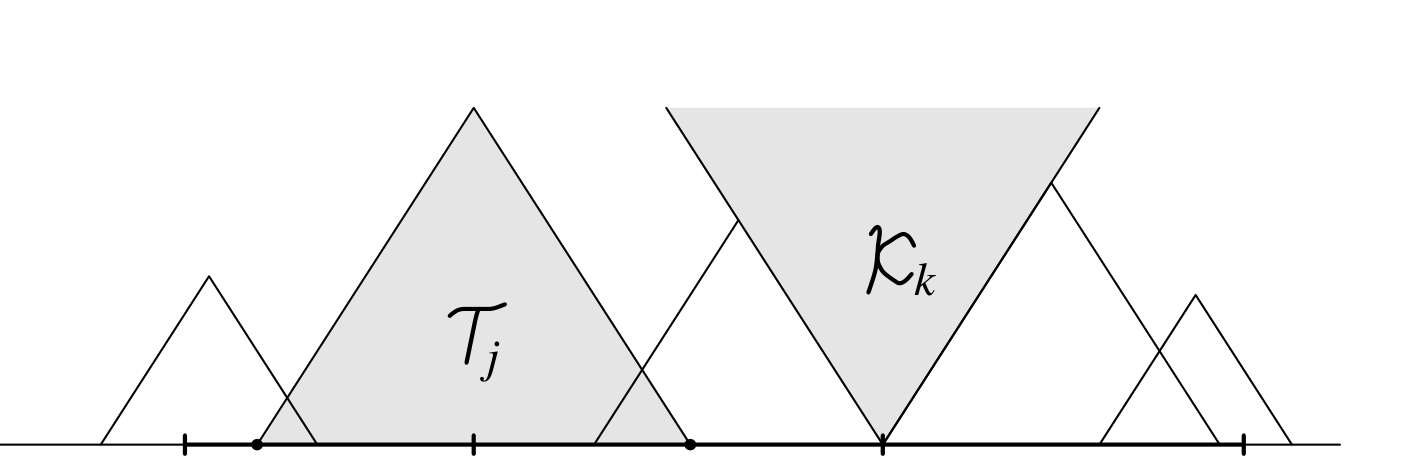
\includegraphics[width=0.85\textwidth]{ch14-fig10-01.png}
\caption{局部近似解的拼接：三角形 $\mathscr{T}_j$ 与扇区 $\mathscr{K}_k$}\label{figure:ch14-局部拼接}
\end{figure}

显然，对充分小的 $h$，$U^*(\cdot,h)$ 对所有 $x\in[a,b]$ 有定义，且
\begin{align}
\int_a^b|U(x,\tau+h)-U^*(x,h)|\,\mathrm{d}x&\leqslant\sum_{k=1}^K\int_{y_k-\lambda h}^{y_k+\lambda h}|U(x,\tau+h)-U^\sharp_{(y_k,\tau)}(x,h)|\,\mathrm{d}x\nonumber\\
&\quad+\sum_{j=1}^J\int_{\zeta_j+\lambda h}^{\xi_j-\lambda h}|U(x,\tau+h)-U^\flat_{(z_j,\tau)}(x,h)|\,\mathrm{d}x.
\label{align:ch14-Ustar-bound}
\end{align}
结合\eqref{align:ch14-Ustar-bound}、\eqref{align:ch14-sector-limit}、\eqref{align:ch14-linear-est}与\eqref{align:ch14-tame}，我们得到\eqref{align:ch14-Ustar1}，其中 $c_{14}=2cc_{15}$。

现注意 $S_{t-\tau}U(\cdot,\tau)$ 对 $t\geqslant\tau$ 定义了\eqref{align:ch14-system}的另一解，它具有相同界，并在 $t=\tau$ 处与 $U$ 相同。因而此解必同样满足\eqref{align:ch14-Ustar1}的类比，即\eqref{align:ch14-Ustar2}。最后，\eqref{align:ch14-Ustar1}与\eqref{align:ch14-Ustar2}一起给出\eqref{align:ch14-tangent}。

还须证明\eqref{align:ch14-tangent}蕴含\eqref{align:ch14-un-trajectory}。为此固定 $t>0$ 与任意小 $\varepsilon>0$。由\eqref{align:ch14-tangent}与 Vitali 覆盖定理，$[0,t]$ 中存在有限两两不交闭子区间 $[\tau_k,\tau_k+h_k]$，$k=1,\cdots,K$，$0\leqslant\tau_1<\cdots<\tau_K<t$，使 $\tau_k\notin\mathscr{N}$ 且
\begin{align}
0\leqslant t-\sum_{k=1}^K h_k<\varepsilon,
\label{align:ch14-vitali}
\end{align}
\begin{align}
\|U(\cdot,\tau_k+h_k)-S_{h_k}U(\cdot,\tau_k)\|_{L^1(-\infty,\infty)}<\varepsilon h_k,\qquad k=1,\cdots,K.
\label{align:ch14-vitali2}
\end{align}
由三角不等式，
\begin{align}
\|U(\cdot,t)-S_tU_0(\cdot)\|_{L^1(-\infty,\infty)}&\leqslant\sum_{k=0}^K\|S_{t-\tau_{k+1}}U(\cdot,\tau_{k+1})-S_{t-\tau_k-h_k}U(\cdot,\tau_k+h_k)\|_{L^1(-\infty,\infty)}\nonumber\\
&\quad+\sum_{k=1}^K\|S_{t-\tau_k-h_k}U(\cdot,\tau_k+h_k)-S_{t-\tau_k}U(\cdot,\tau_k)\|_{L^1(-\infty,\infty)}.
\label{align:ch14-triangle}
\end{align}
在\eqref{align:ch14-triangle}右端第一个和中，$\tau_0+h_0$ 解释为 $0$，$\tau_{K+1}$ 解释为 $t$。此和中的一般项以 $\kappa(1+c'r)(\tau_{k+1}-\tau_k-h_k)$ 为界（由\eqref{align:ch14-semigroup-lip}与\eqref{align:ch14-un-lip}）。因而第一个和以 $\kappa(1+c'r)\varepsilon$ 为界（由\eqref{align:ch14-vitali}）。现在转向第二个和，由于 $S_{t-\tau_k}=S_{t-\tau_k-h_k}S_{h_k}$，
\begin{align}
\|S_{t-\tau_k-h_k}U(\cdot,\tau_k+h_k)-S_{t-\tau_k}U(\cdot,\tau_k)\|_{L^1(-\infty,\infty)}\leqslant\kappa\varepsilon h_k,
\label{align:ch14-second-sum}
\end{align}
由\eqref{align:ch14-semigroup-lip}与\eqref{align:ch14-vitali2}。因而第二个和以 $\kappa t\varepsilon$ 为界。于是\eqref{align:ch14-triangle}右端可任意小，这建立了\eqref{align:ch14-un-trajectory}。证明完成。
\end{proof}

\end{document}
